\documentclass{article}

% Load amsmath first so the style's author separator \And takes precedence.
\usepackage{amsmath,amssymb}
\usepackage[preprint]{neurips_2025}
\usepackage[utf8]{inputenc}
\usepackage[T1]{fontenc}
\usepackage{booktabs,tabularx,array}
\usepackage{microtype}
\usepackage{graphicx}
\usepackage{enumitem}
\usepackage{hyperref}

\newcolumntype{Y}{>{\raggedright\arraybackslash}X}
\newcolumntype{P}[1]{>{\raggedright\arraybackslash}p{#1}}
\setlist[enumerate]{leftmargin=1.8em,itemsep=2pt,topsep=2pt}
\hypersetup{
  colorlinks=true,
  linkcolor=blue,
  citecolor=blue,
  urlcolor=blue,
  pdftitle={PeerSieve: Sketch-Filtered Compressed Streaming for Byzantine-Resilient Decentralized LLM Tuning},
  pdfauthor={Natthanan Bhukan and Germain Dal}
}

\neuripsnotice{Course Project Proposal: Reliable Systems, Tsinghua University.}
\title{PeerSieve: Sketch-Filtered Compressed Streaming\\for Byzantine-Resilient Decentralized LLM Tuning}

\author{%
  Natthanan Bhukan \\
  Tsinghua University \\
  2025280434 \\
  \href{mailto:panyx25@mails.tsinghua.edu.cn}{\texttt{panyx25@mails.tsinghua.edu.cn}} \\
  \And
  Germain Dal \\
  Tsinghua University \\
  2025280175 \\
  \href{mailto:xhm25@mails.tsinghua.edu.cn}{\texttt{xhm25@mails.tsinghua.edu.cn}} \\
}

\begin{document}
\raggedbottom
\maketitle

\begin{abstract}
Decentralized federated learning lets peers fine-tune a language model without a central server, but each receiver must decide which neighbor updates to trust. Downloading full updates before scoring them makes even rejected updates expensive. We propose \textbf{PeerSieve}, which screens small CountSketch announcements before requesting blockwise INT4 payloads. The receiver audits one staged payload at a time and caps each accepted update's magnitude using its own local update. The receive-side tensor buffers do not grow with neighbor count. The audit can detect sketch mismatches and some forms of poisoning, but a matching sketch is not proof of an honest update. We plan to reproduce TrustGraph-DFL on CIFAR-10 and evaluate PeerSieve on an eight-GPU TinyLlama-1.1B benchmark using Dolly-15k. All performance figures are projections, not benchmark results.
\end{abstract}

\section{Motivation and Contribution}
\label{sec:motivation}

In decentralized federated learning (DFL), each peer aggregates updates from its neighbors instead of sending them to a central server. Byzantine neighbors can exploit this exchange to inject poisoned updates. TrustGraph-DFL~\cite{trustgraph2026}, like FLTrust~\cite{cao2021fltrust}, uses a clean local signal to score a neighbor's update. BALANCE~\cite{fang2024balance} instead filters received models by their distance from the receiver's own model. These checks require receiving the update or model before filtering. In the batched TrustGraph-DFL implementation we model, the receiver also holds the entire set of updates before aggregating. Streaming dense updates is possible, but would not reduce network traffic.

For rank-128 LoRA in our TinyLlama example, one FP32 update is 385~MiB. The cost is substantially higher for full-parameter tuning. Savings from early rejection and compression will be largest when the network is slower than local training. Sparse Top-$k$ encoding~\cite{karimireddy2019efsgd} is another option, but selected coordinates may align poorly with a receiver's validation direction on non-IID data. We test that hypothesis rather than assuming sparse updates always fail. A compact sketch also loses information, and removing suspect links can disconnect honest peers. Figure~\ref{fig:story} contrasts these trade-offs.

\begin{figure}[tbp]
  \centering
  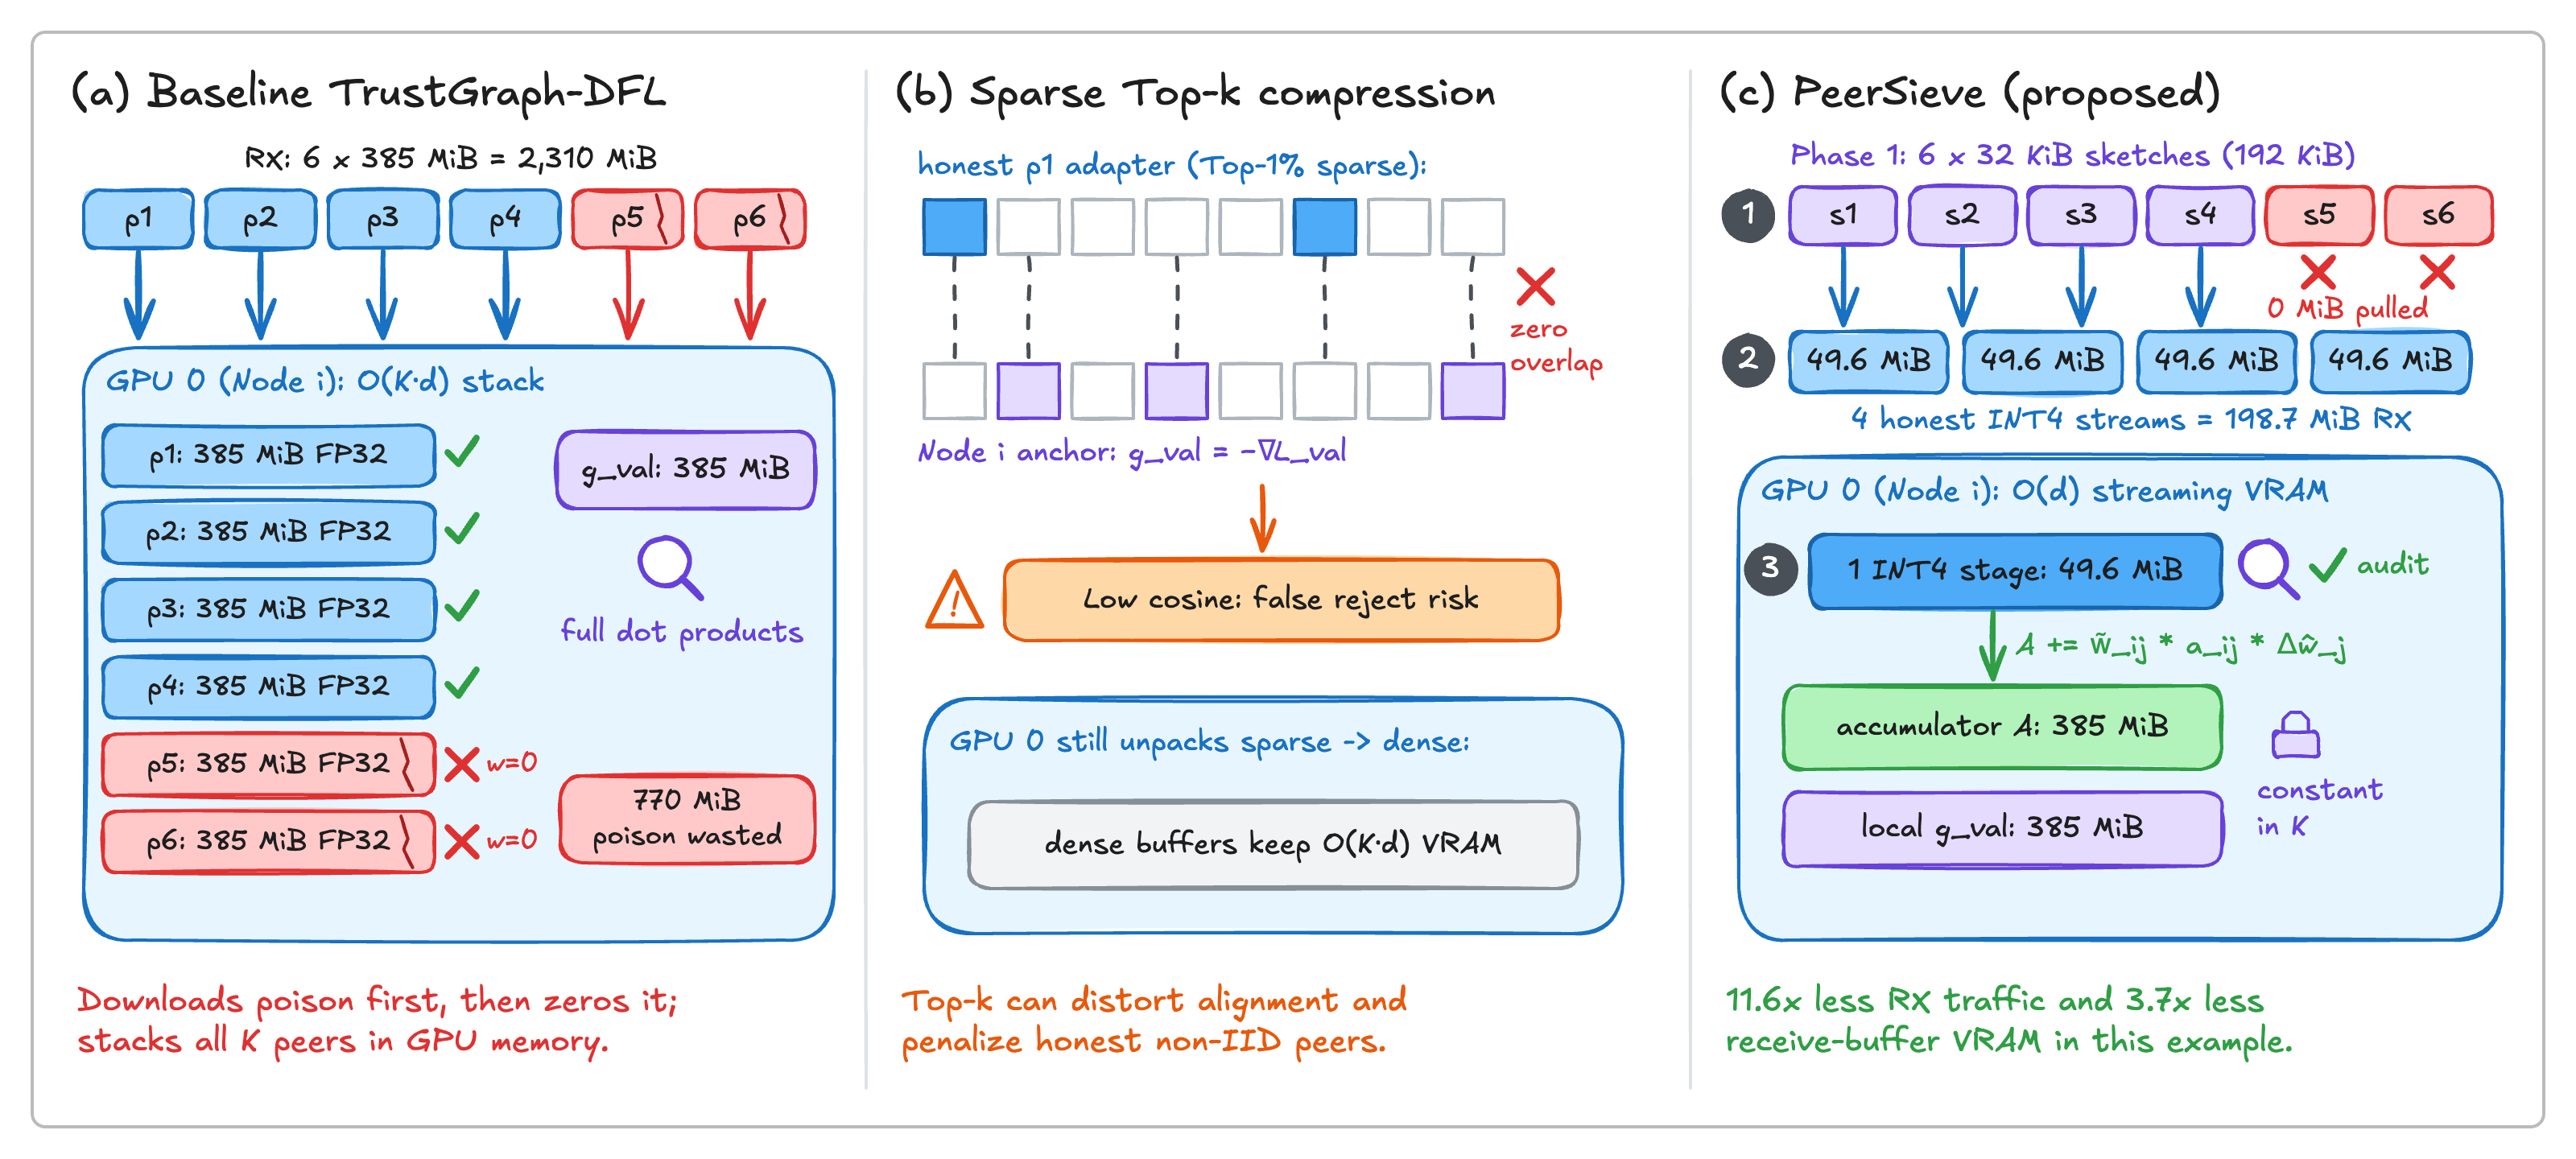
\includegraphics[width=\linewidth]{figures/fig1_story.png}
  \caption{Design comparison for the running example. The batched FP32 baseline receives and stores all updates. Sparse Top-$k$ can distort cosine scores under heterogeneous data. PeerSieve screens sketches before requesting compressed payloads.}
  \label{fig:story}
\end{figure}

PeerSieve makes four contributions:
\begin{enumerate}
  \item Blockwise INT4 encoding with error feedback to reduce transferred bytes while retaining useful directional information.
  \item A two-phase round using CountSketch~\cite{charikar2004countsketch,rothchild2020fetchsgd} to decide which payloads to request.
  \item A two-pass streaming audit that verifies each staged update before accumulation and clips its magnitude without another dense buffer.
  \item Per-edge quarantine with reversible probation and best-effort two-hop neighbor discovery.
\end{enumerate}

\section{Scope and Security-Memory Contract}
\label{sec:scope}

We target synchronous instruction tuning of TinyLlama-1.1B~\cite{zhang2024tinyllama} on Dolly-15k~\cite{conover2023dolly}, using low-rank adaptation (LoRA)~\cite{hu2022lora} or full-parameter updates. Peers use \texttt{torch.distributed} point-to-point transport and a token-bucket limiter to emulate the receiver bandwidth. Table~\ref{tab:scope} states the scope.

\begin{table}[tbp]
  \caption{System scope and trust assumptions.}
  \label{tab:scope}
  \centering\small
  \begin{tabularx}{\linewidth}{@{}P{0.19\linewidth}Y@{}}
    \toprule
    Dimension & Scope \\
    \midrule
    Workload & Non-IID Dolly-15k on 8 peers in the main experiment, up to 16 for the degree sweep. TinyLlama-1.1B with rank-32 LoRA, rank-128 LoRA, or full tuning. \\
    Threat model & Up to two of six neighbors are Byzantine in the main setting and up to three in the stress setting. The round's sketch seed is public. \\
    Trusted state & Each honest receiver trusts its own training and validation data, random number generator, round counter, and transport state. Peer identities are fixed and authenticated for the run. \\
    Compression & Packed blockwise INT4 with 128 elements and one FP16 scale per block, plus a local FP32 error-feedback residual. \\
    Verification & A 32~KiB FP16 sketch screen followed by payload-format, sketch, alignment, and norm checks. \\
    Topology guard & Reversible per-edge probation and best-effort two-hop referral when observed active degree falls below two. \\
    Exclusions & Asynchronous staleness, Sybil identities, corrupted local validation data, hardware bit flips, and guarantees under an eclipsed or disconnected honest graph. \\
    \bottomrule
  \end{tabularx}
\end{table}

\textbf{I1 (verified accumulation).} No received payload changes the running aggregate before it has passed all of the audit checks. Passing those checks does not establish that a peer is honest.

\textbf{I2 (bounded tensor buffers).} The receiver holds one compressed staging buffer, one dequantization tile, its validation direction, and one accumulator. These buffers do not grow with degree. Per-edge metadata may grow with degree.

\textbf{I3 (bounded receive cost on hard faults).} Only requested, size-bounded payloads are staged. After a hard protocol failure the receiver refuses further transfers from that authenticated peer for the run. The bound is one hard-failing payload per sender and receiver, not one malicious transfer across all rounds or receivers.

\textbf{I4 (recoverable suspicion).} A low alignment score or a soft audit failure can trigger probation, not a permanent ban. Periodic probes allow the peer to return to the active state.

\section{System Design}
\label{sec:design}

\subsection{Notation and Blockwise Compression}

Let $d$ be the trainable dimension, $K$ the receiver's degree, and $t$ the synchronous round. Peer $j$ trains locally and sends a parameter increment $\Delta w_j^{(t)} = w_j^{(t,\mathrm{after})} - w_j^{(t)}$. Receiver $i$ computes the validation \emph{descent direction} $g_i^{\mathrm{val}} = -\nabla L_i^{\mathrm{val}}(w_i^{(t)})$ at the start of the round. A positive dot product with $g_i^{\mathrm{val}}$ indicates a predicted decrease in validation loss to first order. Using the positive loss gradient with an after-minus-before increment would reverse that interpretation.

The running example uses TinyLlama-1.1B with rank-128 LoRA on seven linear projections in each of 22 layers: $100{,}925{,}440$ trainable parameters, or $385.0$~MiB in FP32. Node $i$ has six neighbors, including two Byzantine peers in the illustration, and a shared receive budget of $1$~Gb/s.

For each of $788{,}480$ blocks of 128 elements, the sender adds its previous residual and computes the quantizer in Equation~\eqref{eq:quant}. Let $s_b$ be the largest absolute entry divided by seven, rounded to the transmitted FP16 scale. The sender uses that same scale to compute both the decoded update and its new residual. A zero scale encodes an all-zero decoded block.
\begin{equation}
\begin{aligned}
  u_{j,b}^{(t)} &= \Delta w_{j,b}^{(t)} + e_{j,b}^{(t)}, \\
  q_{j,b}^{(t)} &= \operatorname{clip}\!\left(\operatorname{round}\!\left(u_{j,b}^{(t)}/s_b\right),-7,7\right),
                   \qquad s_b>0, \\
  y_{j,b}^{(t)} &= s_b q_{j,b}^{(t)}, \qquad
  e_{j,b}^{(t+1)} = u_{j,b}^{(t)} - y_{j,b}^{(t)} .
\end{aligned}
\label{eq:quant}
\end{equation}

Figure~\ref{fig:compress} shows the encoder. The receiver decodes exactly the same vector $y_j^{(t)}$ (denoted $\widehat{\Delta w}_j^{(t)}$ in the figures). The encoded block is 66~B versus 512~B in FP32, so the full payload is 49.63~MiB. In a synthetic Gaussian-block check, the mean cosine between the quantizer input and decoded block was approximately $0.993$. Alignment on recorded LoRA updates remains to be measured. Error feedback carries the quantization residual into the next local update. It does not compensate for rejection or receiver-side clipping.

\begin{figure}[tbp]
  \centering
  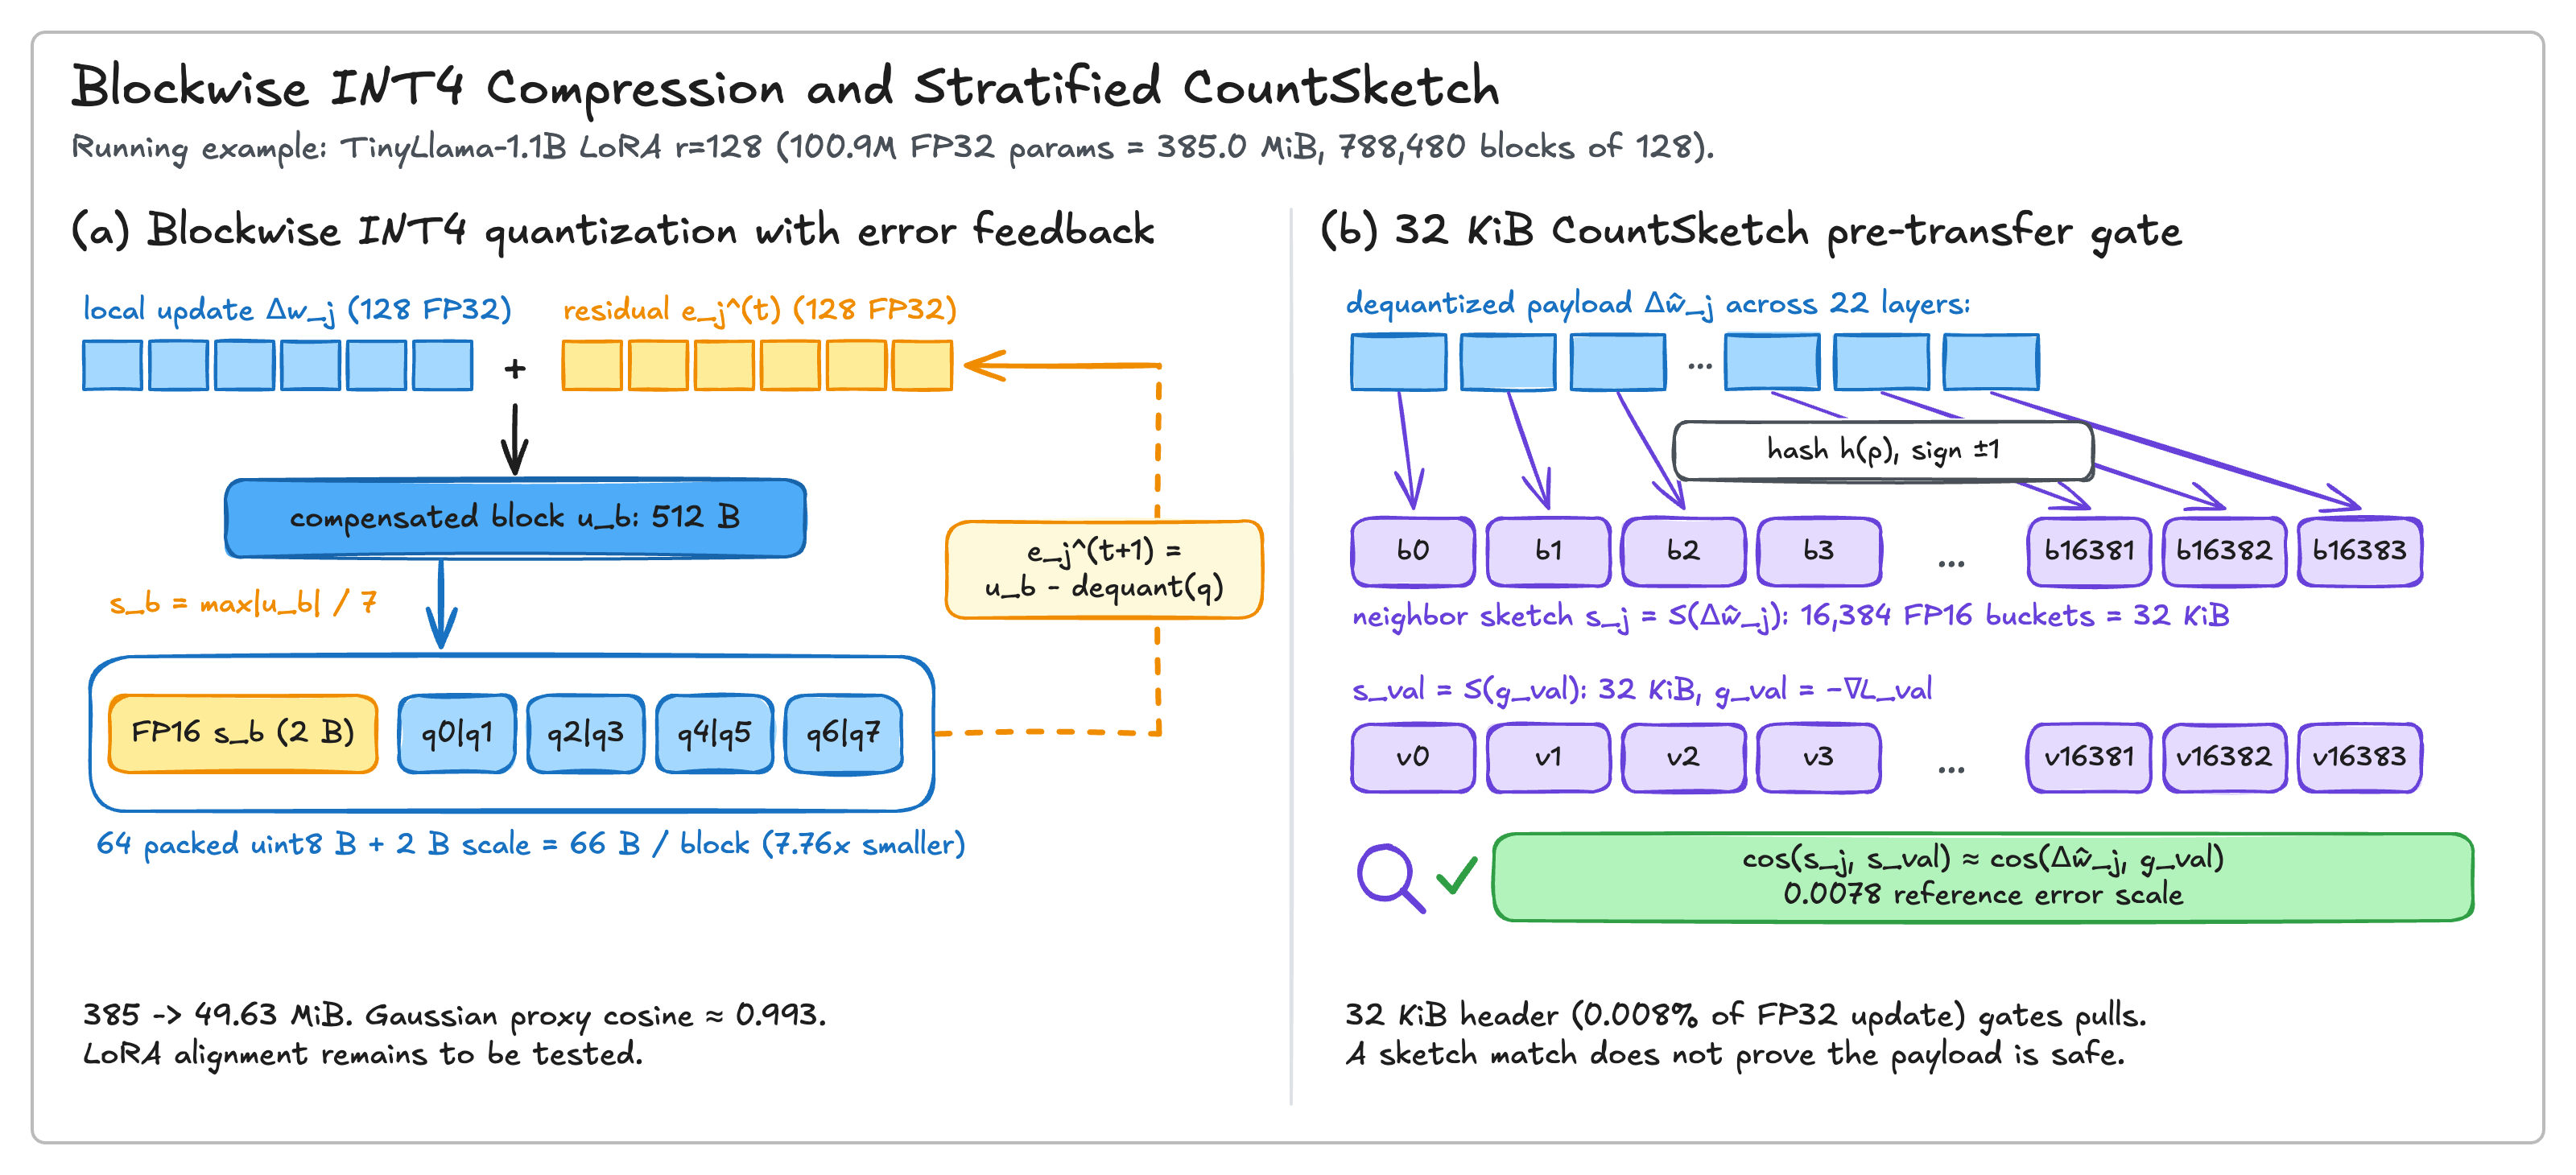
\includegraphics[width=\linewidth]{figures/fig2_compress.png}
  \caption{Each 128-element block uses 64 packed INT4 bytes and a two-byte FP16 scale, a $7.76\times$ reduction relative to FP32. The sender sketches the decoded update, not the original FP32 update.}
  \label{fig:compress}
\end{figure}

\subsection{Sketch-Based Screening}

The ideal CountSketch $\mathcal S_t$ maps the $d$ coordinates into $m=16{,}384$ signed buckets, partitioned by layer in proportion to each layer's parameter count. Hashes and signs are shared for the round. Let $F_t(v)$ be the result of accumulating $\mathcal S_t(v)$ in FP32 in a specified order and rounding to FP16. The wire format disallows nonfinite values and uses one representation for zero. Sender $j$ announces $s_j^{(t)}=F_t(y_j^{(t)})$, and receiver $i$ computes $s_i^{\mathrm{val}}=F_t(g_i^{\mathrm{val}})$. Using the same decoding and reduction order allows a valid payload to reproduce its announcement.
\begin{equation}
\begin{aligned}
  \widehat c_{ij}^{(t)} &=\frac{\langle s_j^{(t)},s_i^{\mathrm{val}}\rangle}
  {\|s_j^{(t)}\|_2\|s_i^{\mathrm{val}}\|_2}, &
  c_{ij}^{(t)} &=\frac{\langle y_j^{(t)},g_i^{\mathrm{val}}\rangle}
  {\|y_j^{(t)}\|_2\|g_i^{\mathrm{val}}\|_2} .
\end{aligned}
\label{eq:sketch}
\end{equation}

We skip comparisons with zero norms. One FP16 sketch occupies 32~KiB, about $0.008\%$ of the FP32 rank-128 update. Under the usual independent signed hashing assumptions, the ideal sketch's inner product is unbiased for fixed input vectors. The sketched cosine includes random norms and need not be unbiased. The heuristic $m^{-1/2}\approx 0.0078$ is a reference error scale, not a bound. We will measure tail errors with actual updates, the layer allocation, and FP16 rounding.

\subsection{Two-Phase Round Protocol}

Figure~\ref{fig:protocol} shows a modeled round in which both Byzantine neighbors fail the sketch screen and no payload is requested from them. A passing sketch is permission to transfer, not permission to accumulate.

\begin{figure}[tbp]
  \centering
  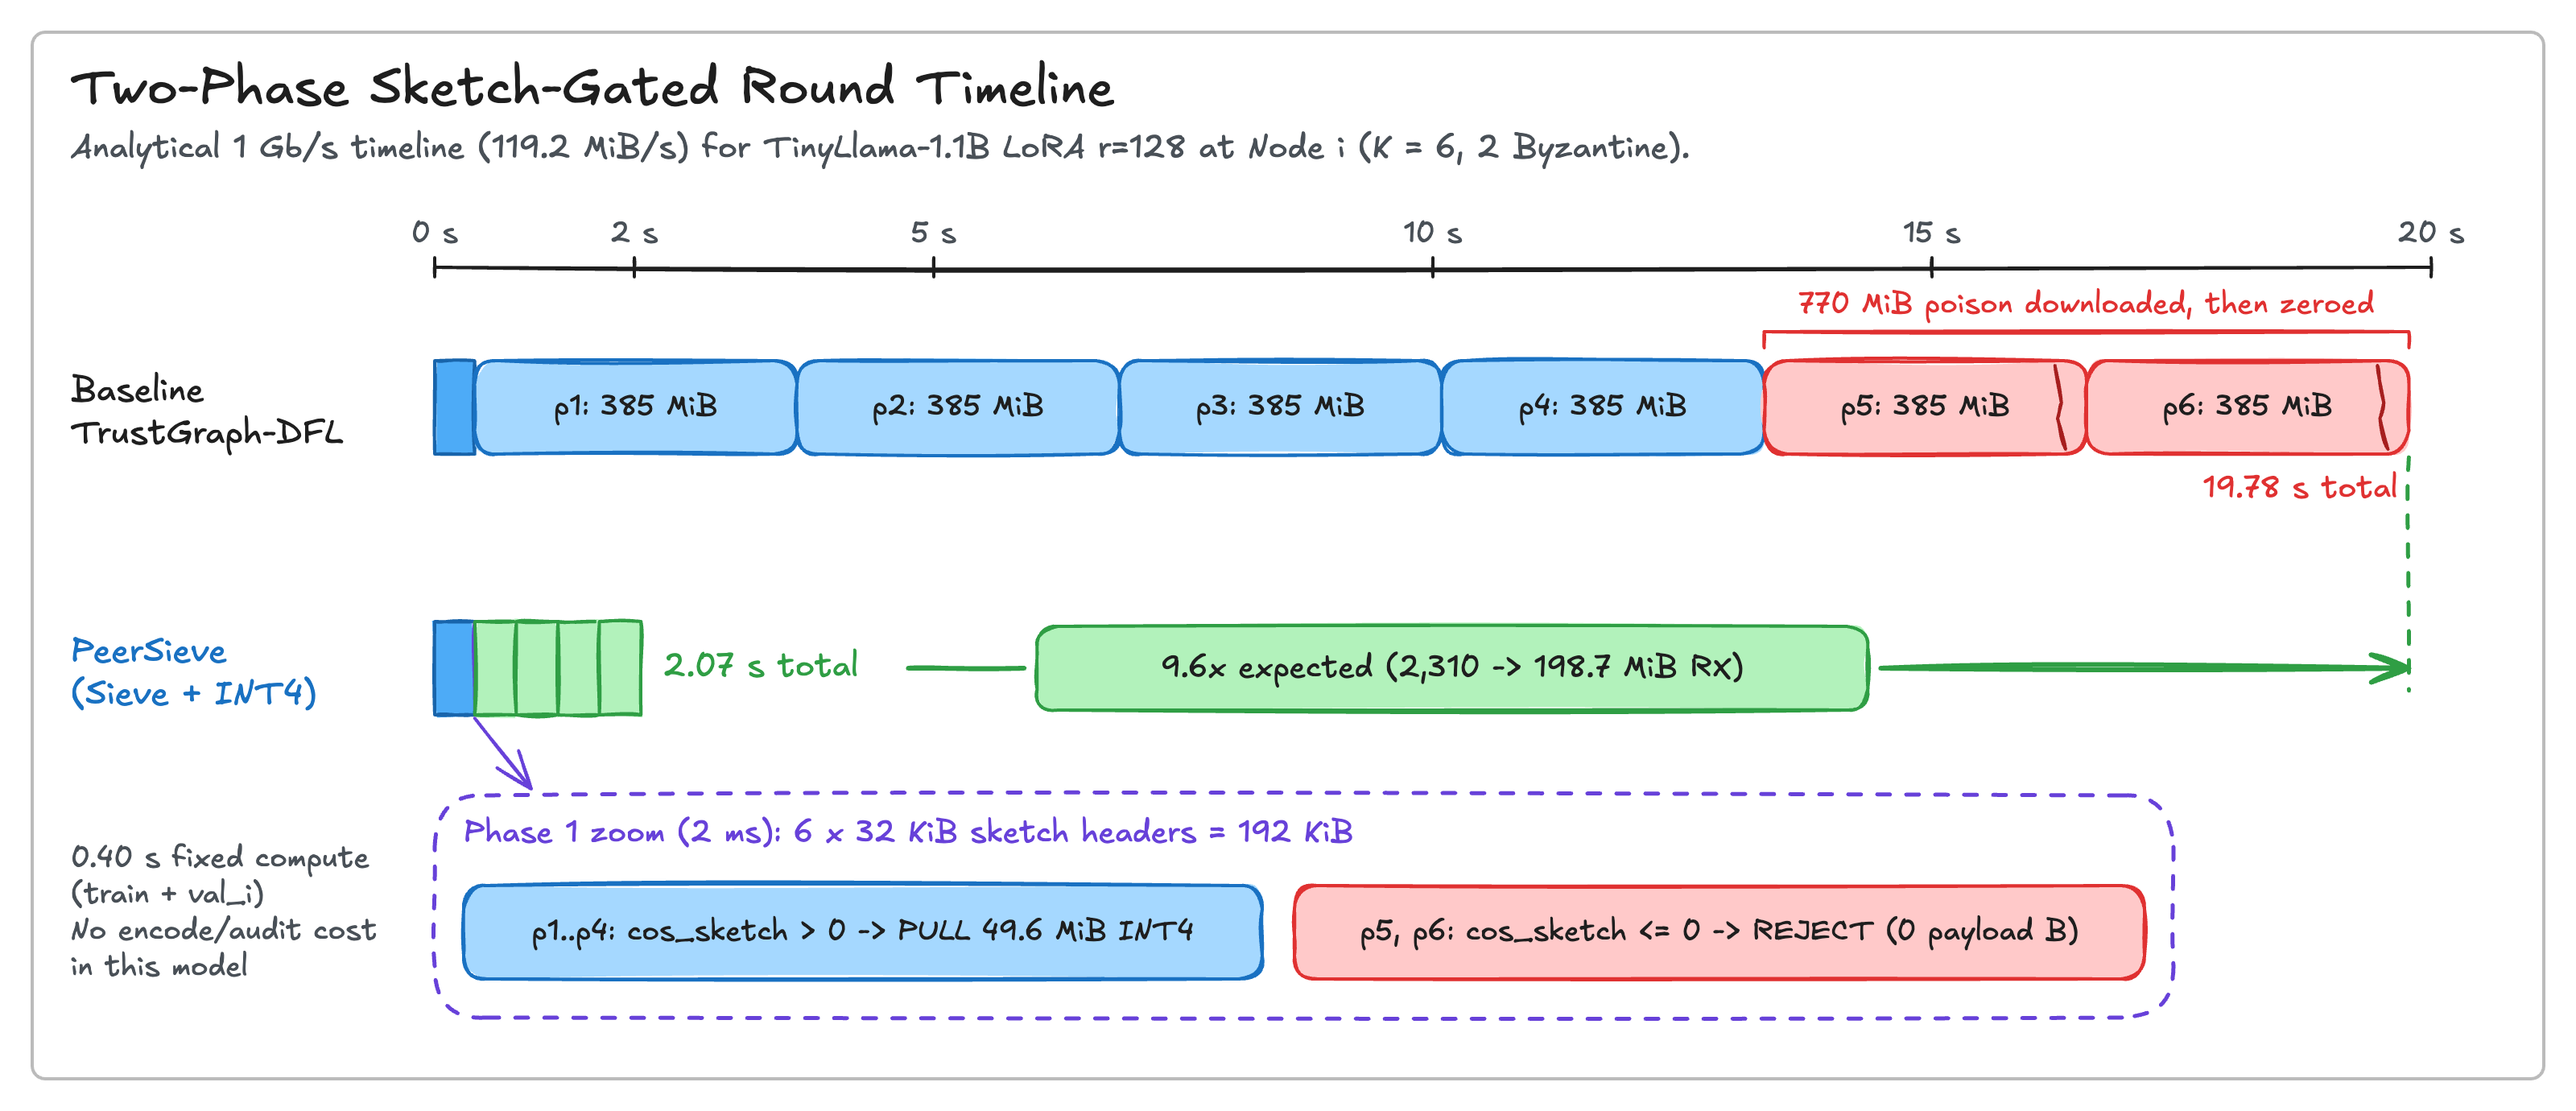
\includegraphics[width=\linewidth]{figures/fig3_protocol.png}
  \caption{Modeled receive timeline at $1$~Gb/s. The FP32 baseline spends 19.38~s receiving six updates. PeerSieve receives six sketches and four 49.63~MiB payloads in this scenario. The model does not include encoding, audit, or transport overhead.}
  \label{fig:protocol}
\end{figure}

\begin{enumerate}
  \item \textbf{Local work.} Node $i$ computes its validation direction and sketch, runs four local optimizer steps, then encodes and sketches its increment.
  \item \textbf{Announce.} Each active peer sends a fixed-size message bound to its authenticated identity, run, and round. Six sketch bodies total 192~KiB (about 1.6~ms at $1$~Gb/s). Probation probes follow Section~\ref{sec:quarantine}.
  \item \textbf{Screen.} The receiver requests a payload only when the announced sketch scores strictly positive under Equation~\eqref{eq:sketch}.
  \item \textbf{Transfer and audit.} Each request allows one size-bounded receive for that peer and round. The receiver stages and verifies one payload at a time (Section~\ref{sec:audit}).
  \item \textbf{Aggregate.} The receiver normalizes the accumulated neighbor update once at the end of the round and updates the edge states.
\end{enumerate}

Table~\ref{tab:round} assumes serial receive at $1$~Gb/s and a fixed 0.40~s local compute budget. The scenario is illustrative: if the sketch screen accepts more peers, PeerSieve transfers more payloads. None of the times include encoding, auditing, or other protocol overhead.

\begin{table}[tbp]
  \caption{Modeled costs for rank-128 LoRA at degree six, with two rejected Byzantine peers for PeerSieve. VRAM is for receive-side tensor buffers only. The Top-1\% row assumes 8~B per nonzero and a receiver that expands sparse updates into dense buffers.}
  \label{tab:round}
  \centering\small
  \begin{tabularx}{\linewidth}{@{}Yrrr@{}}
    \toprule
    Configuration & RX (MiB) & RX + compute (s) & RX VRAM (MiB) \\
    \midrule
    Batched TrustGraph-DFL (FP32) & 2,310.0 & 19.78 & 3,080.0 \\
    Sparse Top-1\% + TrustGraph & 46.2 & Not modeled & 3,080.0 \\
    Blockwise INT4, no sketch gate & 297.8 & 2.90 & 3,080.0 \\
    PeerSieve, gate before quarantine & 198.7 & 2.07 & 823.6 \\
    PeerSieve, four active edges & 198.6 & 2.07 & 823.6 \\
    \bottomrule
  \end{tabularx}
\end{table}

\subsection{Streaming Aggregation and Payload Audit}
\label{sec:audit}

A positive cosine score alone does not constrain magnitude. Neither the original cosine checks nor the sketch-to-payload norm ratio penalize uniformly scaling an update and its announcement in exact arithmetic. We therefore bound the decoded vector before adding it. Inspired by FLTrust's magnitude normalization~\cite{cao2021fltrust}, we use an upper cap rather than rescaling small updates upward. Let $r_i^{(t)}=\|\Delta w_i^{(t)}\|_2$ be the norm of the receiver's own unclipped, uncompressed increment. The receiver computes this scalar locally, without trusting any sender-reported norm. For nonzero accepted payloads, let
\begin{equation}
\begin{aligned}
  a_{ij}^{(t)} &= \min\!\left(1,\frac{r_i^{(t)}}{\|y_j^{(t)}\|_2}\right), \qquad
  \widetilde w_{ij}^{(t)} = \max\!\left(0,c_{ij}^{(t)}\right), \\
  W_i^{(t)} &= \sum_{j\in\mathcal N_i^{\mathrm{acc}}} \widetilde w_{ij}^{(t)}, \qquad
  \Delta\bar w_i^{(t)} = \frac{1}{W_i^{(t)}}
  \sum_{j\in\mathcal N_i^{\mathrm{acc}}}\widetilde w_{ij}^{(t)} a_{ij}^{(t)} y_j^{(t)} .
\end{aligned}
\label{eq:stream}
\end{equation}
Here $\mathcal N_i^{\mathrm{acc}}$ contains the neighbors whose payloads passed the audit. The denominator sums the trust weights only, not the clipping factors. When $W_i^{(t)}>0$, the triangle inequality gives $\|\Delta\bar w_i^{(t)}\|_2\le r_i^{(t)}$. This caps absolute magnitude, not the fraction of trust assigned to a Byzantine peer. In the LLM experiments we blend the local and neighbor increments with self-weight $0.5$. If $W_i^{(t)}=0$, the receiver keeps its locally trained model without a neighbor step.

\begin{figure}[tbp]
  \centering
  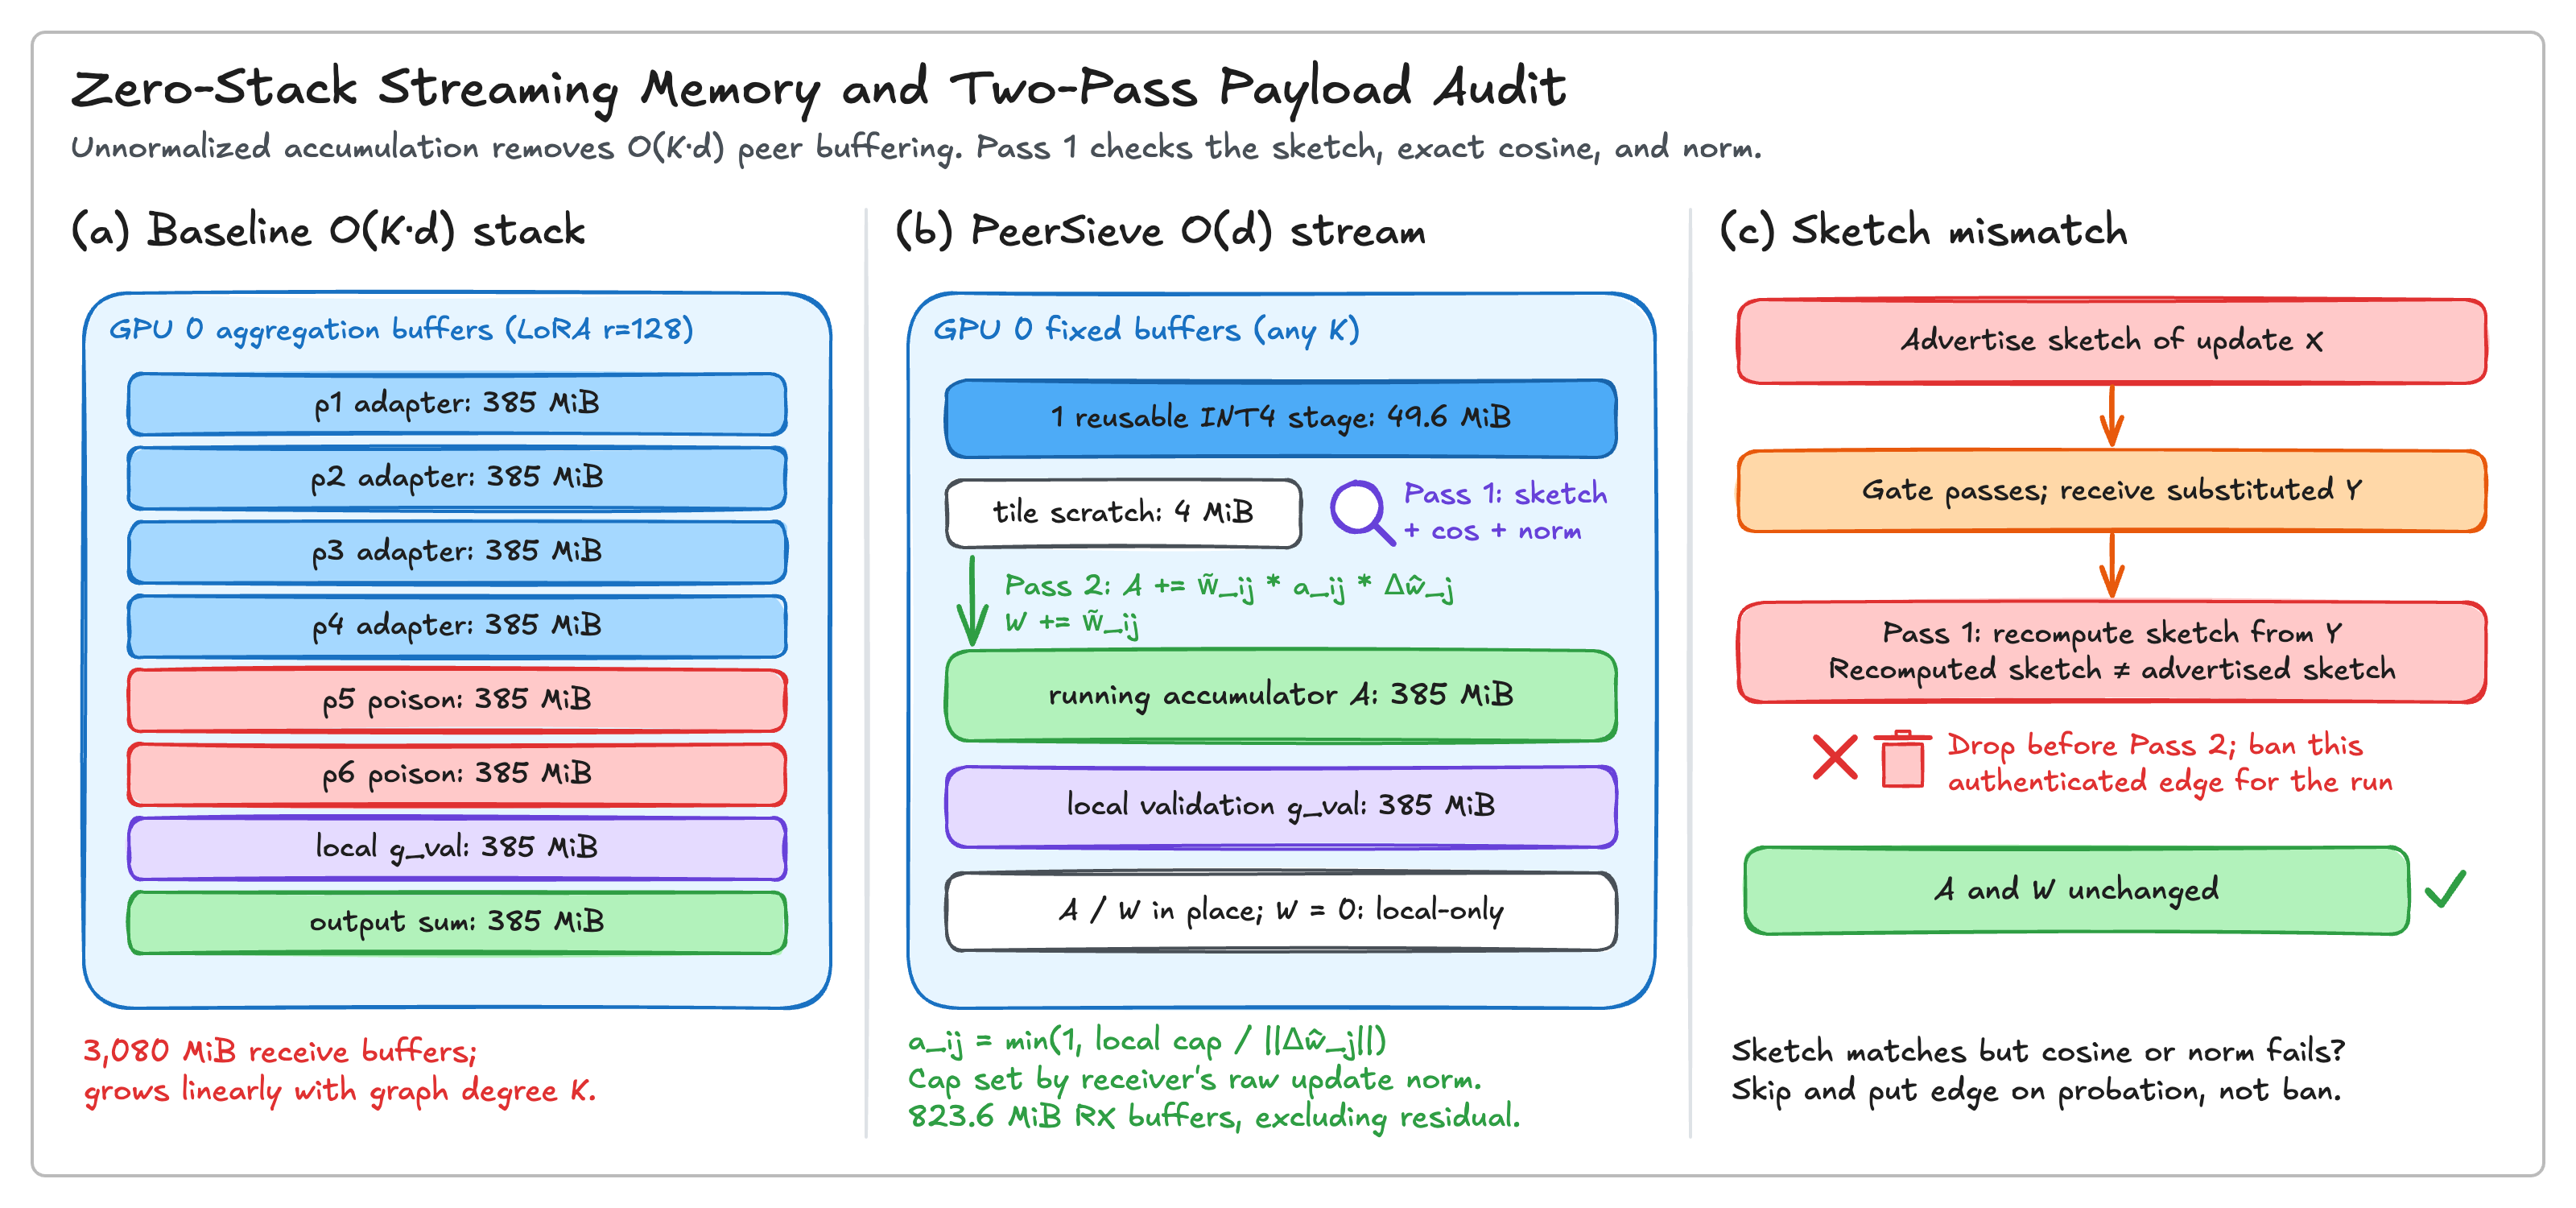
\includegraphics[width=\linewidth]{figures/fig4_stream.png}
  \caption{The batched baseline holds one dense buffer per neighbor. PeerSieve reuses one stage and one tile. Pass~1 audits the payload. Pass~2 runs only on acceptance and adds the clipped, trust-weighted update to the accumulator.}
  \label{fig:stream}
\end{figure}

\textbf{Pass 1: verify without accumulation.} The receiver checks the identity, round, length, and packed format, then decodes in tiles of at most 4~MiB. It recomputes the sketch using $F_t$, calculates the full-vector cosine $c_{ij}^{(t)}$, and measures $\|y_j^{(t)}\|_2$. With well-formed, finite, nonzero inputs, all four conditions must hold:
\begin{equation}
\begin{aligned}
  F_t(y_j^{(t)}) &= s_j^{(t)}, & c_{ij}^{(t)} &> 0, \\
  |\widehat c_{ij}^{(t)}-c_{ij}^{(t)}| &\le \tau_c, &
  \left|\frac{\|s_j^{(t)}\|_2}{\|y_j^{(t)}\|_2}-1\right| &\le \tau_n .
\end{aligned}
\label{eq:audit}
\end{equation}
The starting tolerances are $\tau_c=0.05$ and $\tau_n=0.03$. We will recalibrate them using empirical $99.9$th-percentile discrepancies from separate attack-free runs, then freeze them before evaluation. A protocol fault, such as a malformed encoding or a conflicting canonical sketch, warrants a run-long ban on that edge. Finite alignment or norm disagreement is a soft failure: discard the staged payload and put the edge on probation. A zero update can be skipped without a hard ban.

\textbf{Pass 2: accumulate.} The receiver reads the same, unchanged staging buffer and adds $\widetilde w_{ij}^{(t)} a_{ij}^{(t)}y_j^{(t)}$ tile by tile. It increments $W_i^{(t)}$ only for an accepted payload and divides the numerator in place only if $W_i^{(t)}>0$. Figure~\ref{fig:stream} shows the tensor footprint for fixed $d$ and sketch size.

\textbf{What the audit cannot certify.} A sketch mismatch detects substitution that changes the canonical sketch, not every change to the input. A perturbation in the ideal sketch's nullspace leaves the sketch unchanged. Some such changes increase the norm or disrupt alignment, but a change that preserves the norm and validation alignment can pass the same checks, up to finite-precision effects. There is no general 25\% relative-norm bound from Equation~\eqref{eq:audit}. The evaluation will measure how often these cases pass and how much they affect training. Clipping limits their magnitude once accepted, not their direction.

\subsection{Link Quarantine and Topology Repair}
\label{sec:quarantine}

Not every negative sketch implies poisoning. A single negative sketch skips that payload. Each edge tracks an exponentially weighted moving average (EWMA) of sketch scores, and enters probation after three consecutive rounds with $R_{ij}^{(t)}<0$. Soft audit failures also trigger probation. The smoothing factor is $\beta=0.7$, and the $k$th probation uses the backoff below, capped at $T_{\max}=16$ rounds.
\begin{equation}
  R_{ij}^{(t)}=\beta R_{ij}^{(t-1)}+(1-\beta)\widehat c_{ij}^{(t)}, \qquad
  T_{\mathrm{backoff}}(k)=\min\!\left(2^k,T_{\max}\right) .
\label{eq:backoff}
\end{equation}
A probation edge carries no payload. At expiry a 32~KiB probe that passes the screen restores the edge to active status. A failed probe extends probation. A hard fault blocks further traffic from the peer at this receiver for the duration of the run.

When observed active degree falls below two, the receiver asks its active neighbors for referrals and screens a sketch from an eligible, authenticated candidate. Rewiring respects the initial degree cap and never reinstates a banned peer. An isolated node can still use scheduled probes on probation edges. The procedure is best effort: it needs a reachable candidate and cannot identify which active peers are honest or guarantee the honest graph stays connected.

\begin{figure}[tbp]
  \centering
  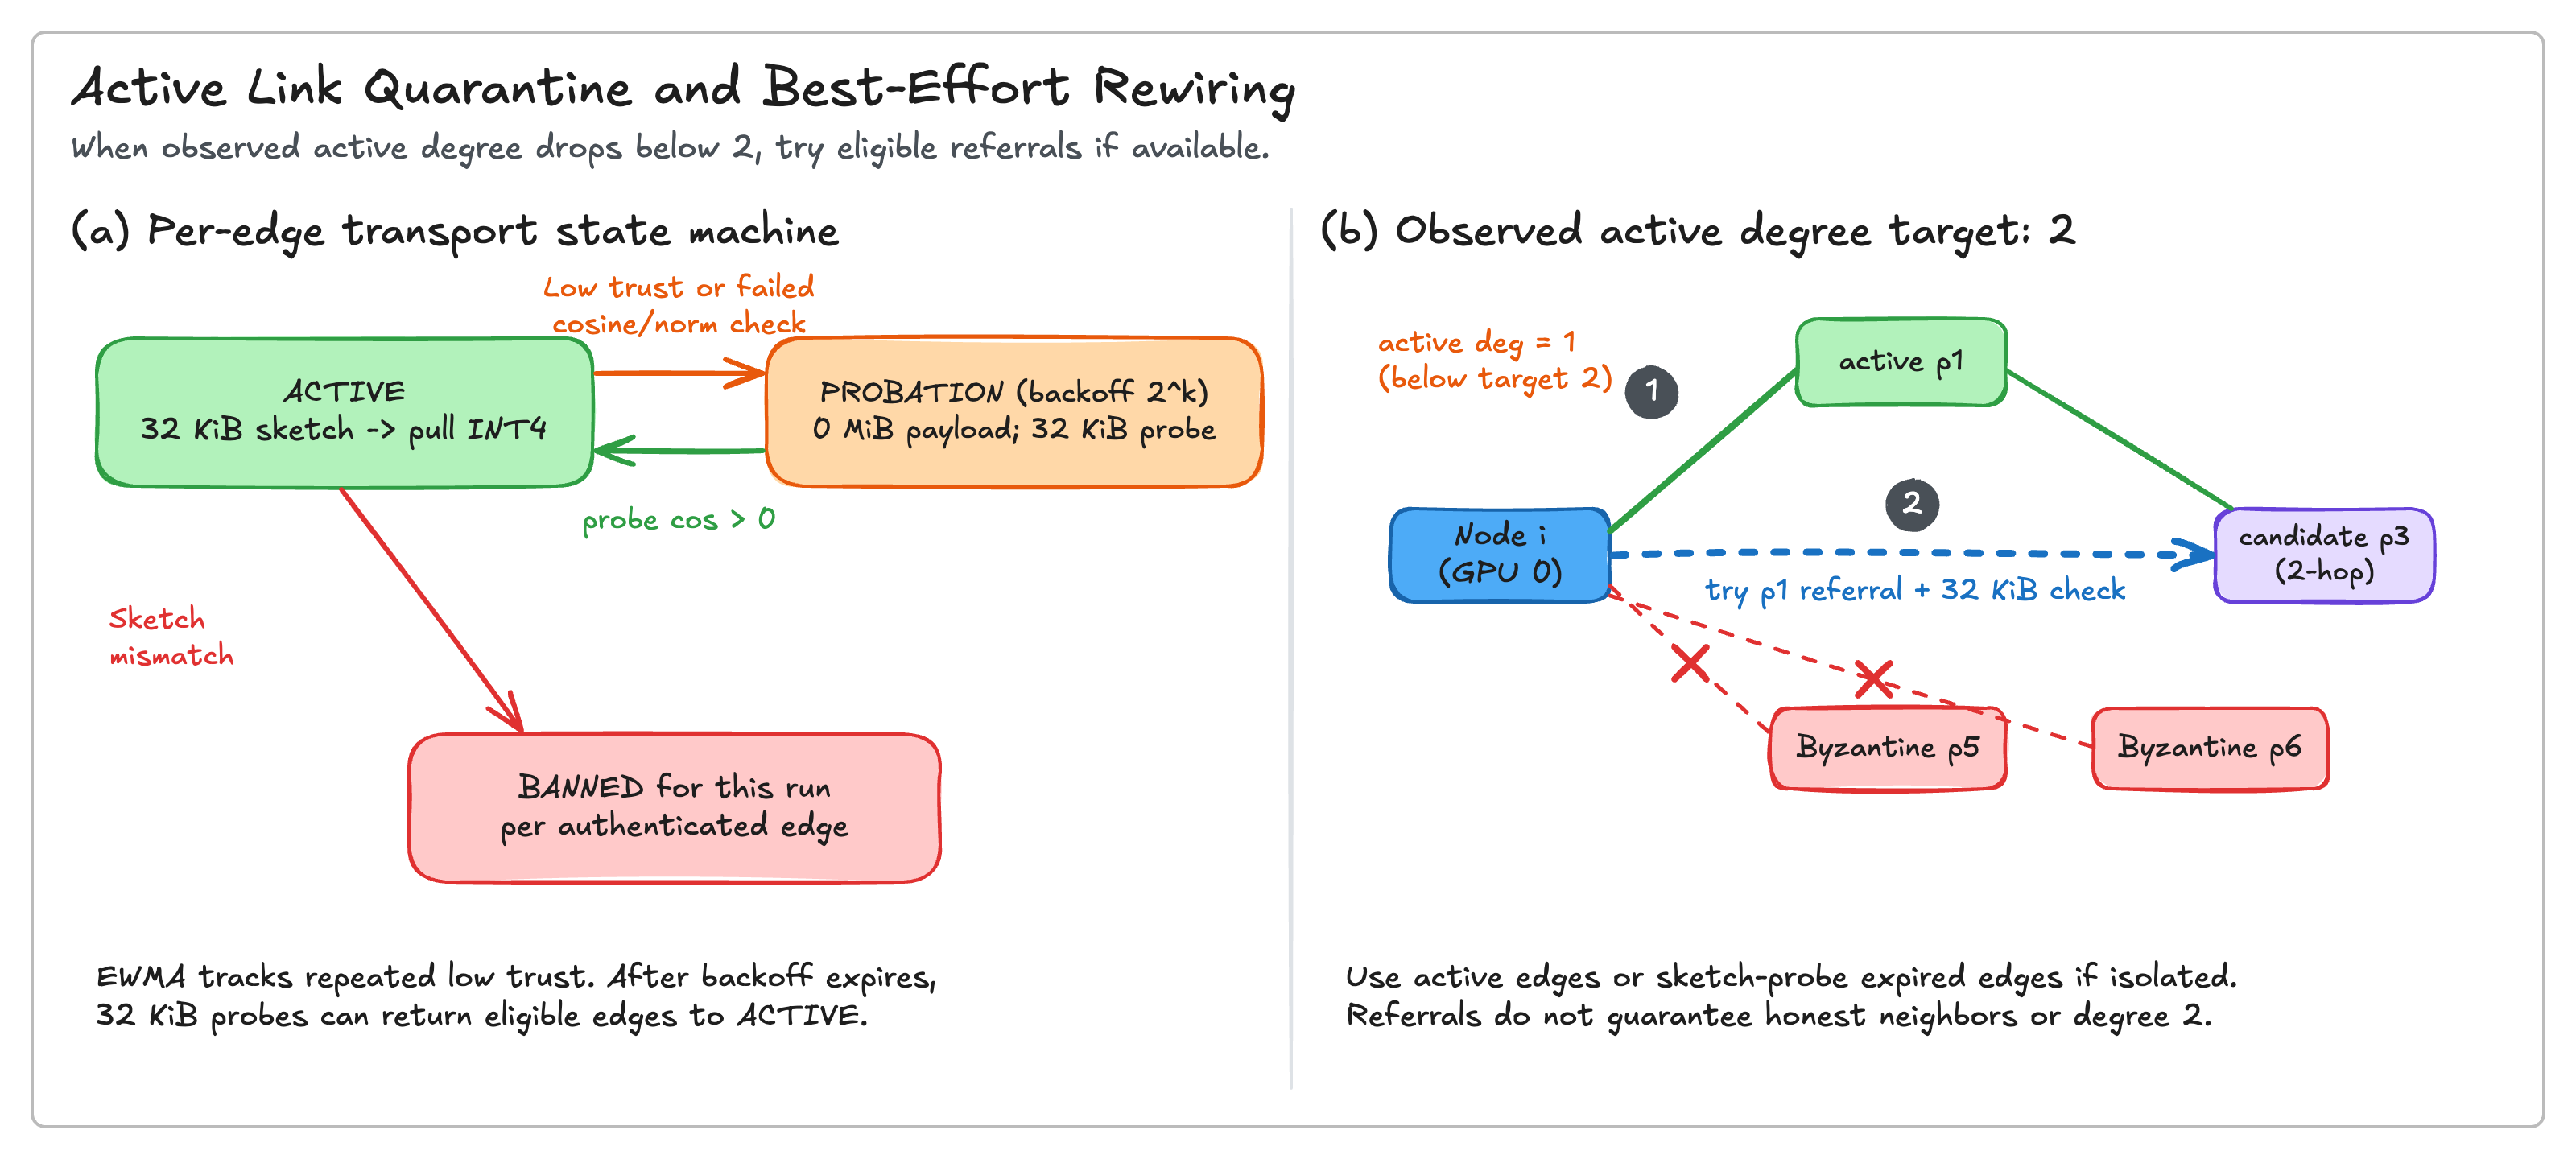
\includegraphics[width=\linewidth]{figures/fig5_quarantine.png}
  \caption{Per-edge state transitions and a successful two-hop referral. The receiver targets an observed active degree of two. Success depends on reachability and candidates passing the screen.}
  \label{fig:quarantine}
\end{figure}

\begin{figure}[tbp]
  \centering
  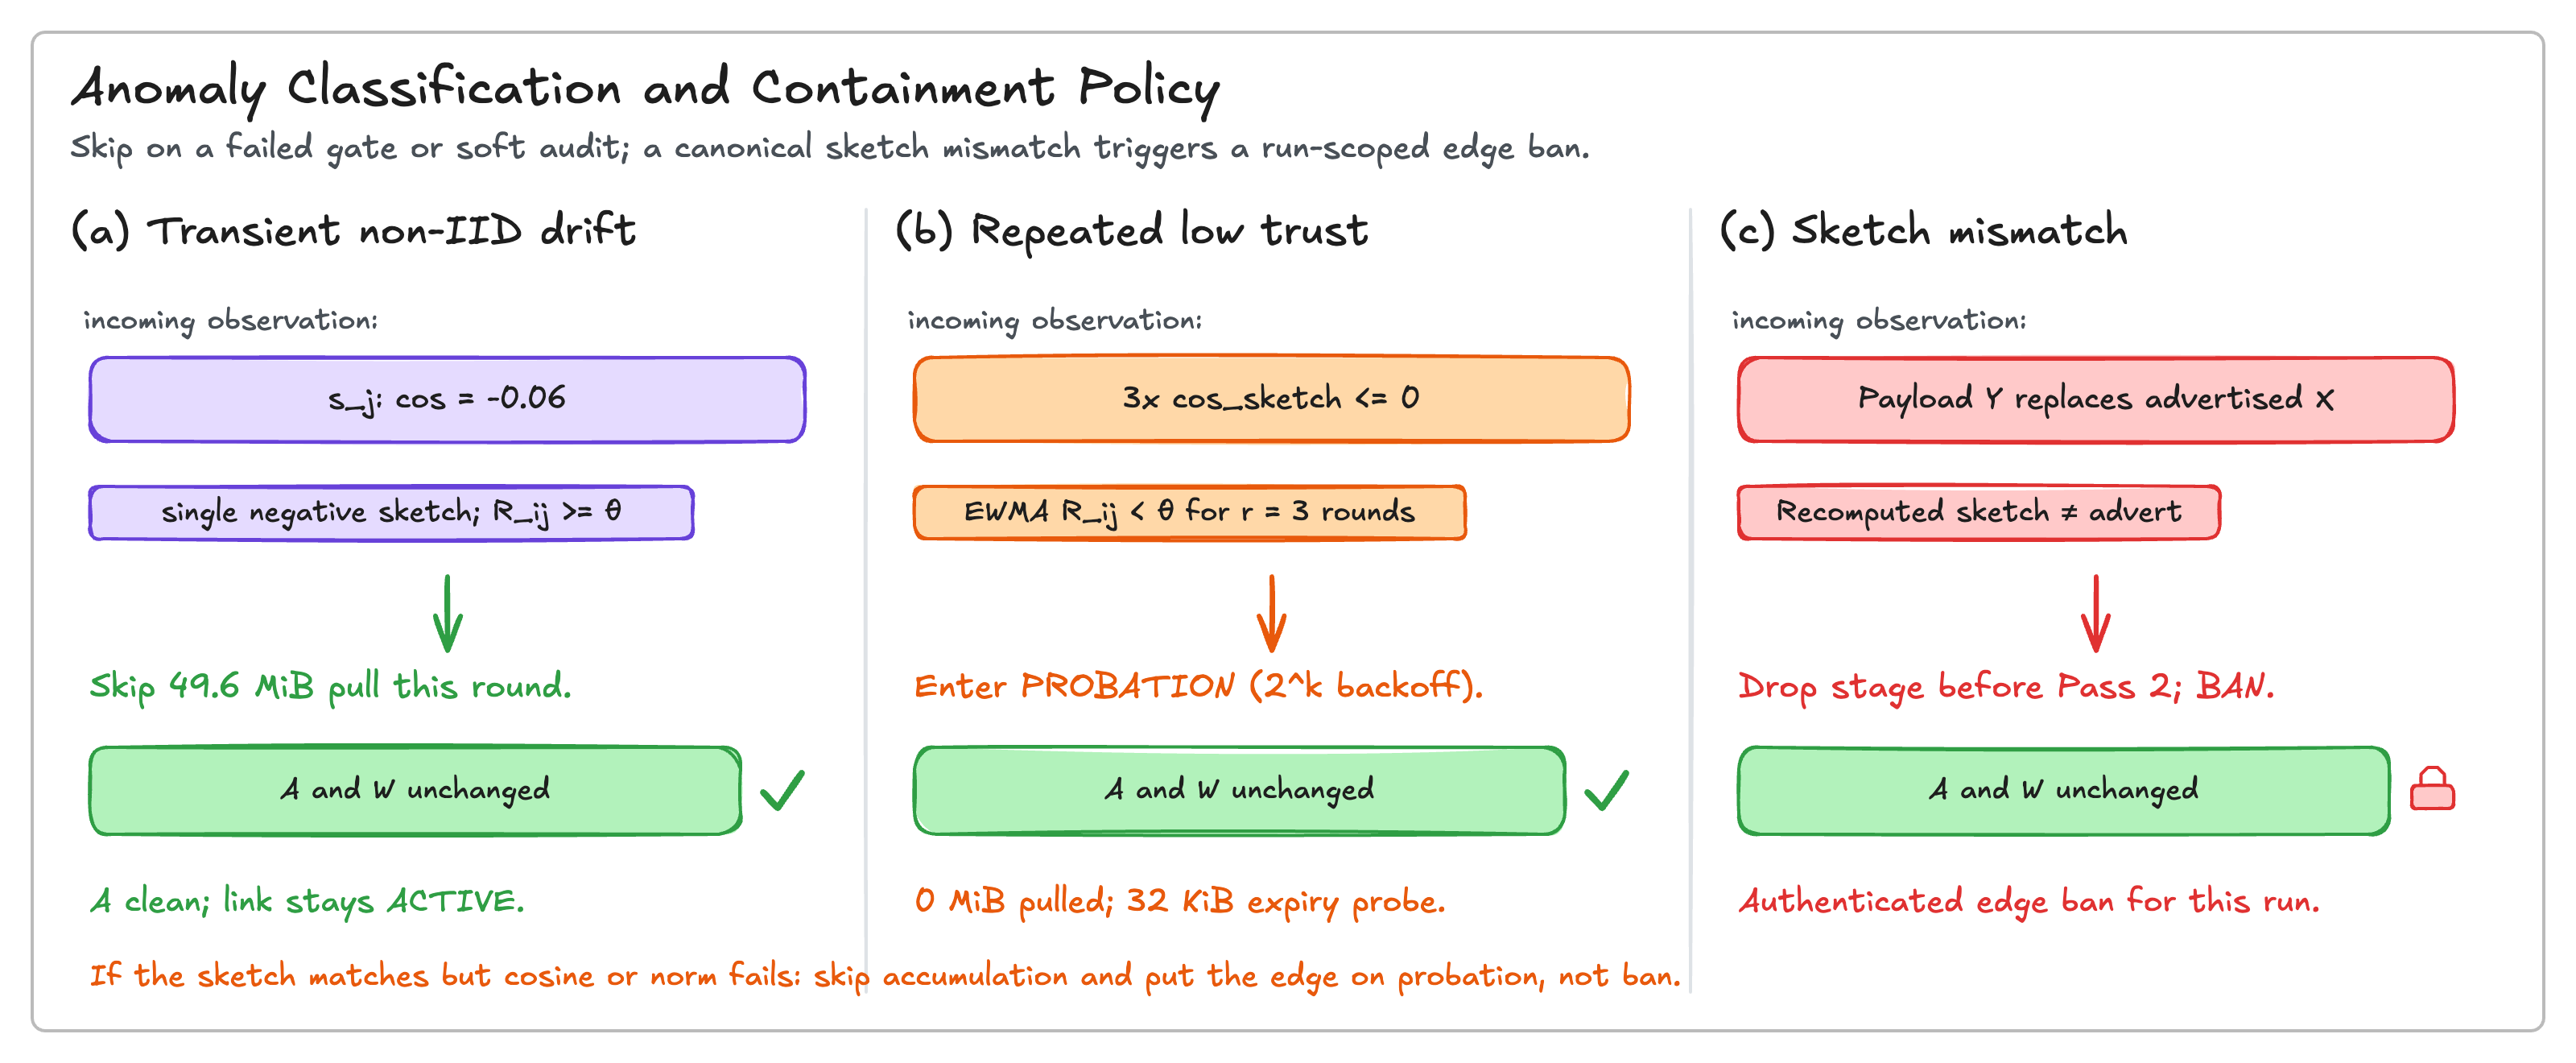
\includegraphics[width=\linewidth]{figures/fig6_policy.png}
  \caption{Containment policy. Transient sketch misalignment skips a pull. Persistent misalignment or a soft audit failure leads to probation. A hard protocol fault, such as a conflicting sketch, leads to a ban. A rejected payload never changes the accumulator.}
  \label{fig:policy}
\end{figure}

Figures~\ref{fig:quarantine} and~\ref{fig:policy} illustrate the state machine and rejection policy. Table~\ref{tab:modules} lists the tests that gate GPU evaluation.

\begin{table}[tbp]
  \caption{Implementation modules and pre-GPU verification gates.}
  \label{tab:modules}
  \centering\small
  \begin{tabularx}{\linewidth}{@{}P{0.23\linewidth}Y Y@{}}
    \toprule
    Module & Mechanism & Verification gate \\
    \midrule
    Blockwise INT4 + error feedback & 128-element packer and FP32 residual. & Check decoded values and residual accounting to floating-point tolerance. Measure cosine on recorded LoRA updates. \\
    CountSketch screen & Layer-stratified, deterministic FP32 reduction and FP16 wire format. & Check sender and receiver agreement across tiling. Measure cosine and norm error on attack-free traces. \\
    Two-pass stream audit & Reusable compressed buffer, tiled decoding, and scalar norm cap. & Failed audits leave both the accumulator and total weight unchanged. Accepted contributions respect the cap. \\
    Quarantine and referral & Authenticated edge states and capped backoff. & Multi-process Gloo tests cover hard-fault bans, soft-fault recovery, and reachability with and without eligible referrals. \\
    \bottomrule
  \end{tabularx}
\end{table}

\section{Evaluation Plan}
\label{sec:eval}

\subsection{Research Questions}

\begin{enumerate}[label=\textbf{RQ\arabic*.}]
  \item \textbf{Accuracy.} Does PeerSieve retain the held-out perplexity and next-token accuracy of uncompressed TrustGraph-DFL under attack?
  \item \textbf{Robustness.} Which poisoned updates pass the screen and audit, how much weight do they receive, and how often do we reject honest peers?
  \item \textbf{Efficiency.} How do round time and bytes received change with link bandwidth and with each mechanism enabled?
  \item \textbf{Memory.} Does the receive-side tensor footprint remain flat across degrees, and can full-parameter tuning fit on one 40~GB A100 per peer?
\end{enumerate}

\subsection{Baseline Reproduction, Testbed, and Configurations}

\textbf{Stage 1: CIFAR-10 reproduction.} We will reimplement the TrustGraph-DFL preprint's 20-node CNN experiment~\cite{trustgraph2026}. We will compare test accuracy against BALANCE at $30\%$ Byzantine nodes and compare honest rejection rates against Krum in its $50\%$ stress setting. The preprint pairs an after-minus-before increment with a positive validation loss gradient in Algorithm~1. We will test the sign as printed and the descent convention from Section~\ref{sec:design}, report any discrepancies with the paper, and use the descent-corrected FP32 implementation as our LLM baseline. We do not assume that either implementation reproduces the paper's reported results.

\textbf{Stage 2: language-model evaluation.} Figure~\ref{fig:eval} shows the planned testbed: eight NVIDIA A100-PCIE-40GB GPUs on \texttt{octave}, using PCIe Gen4 without NVLink. The main configuration places one peer on each GPU in a six-regular graph. We use the same pretrained weights and partition seeds in all configurations. The token bucket controls the total receive rate at each peer.

\begin{figure}[tbp]
  \centering
  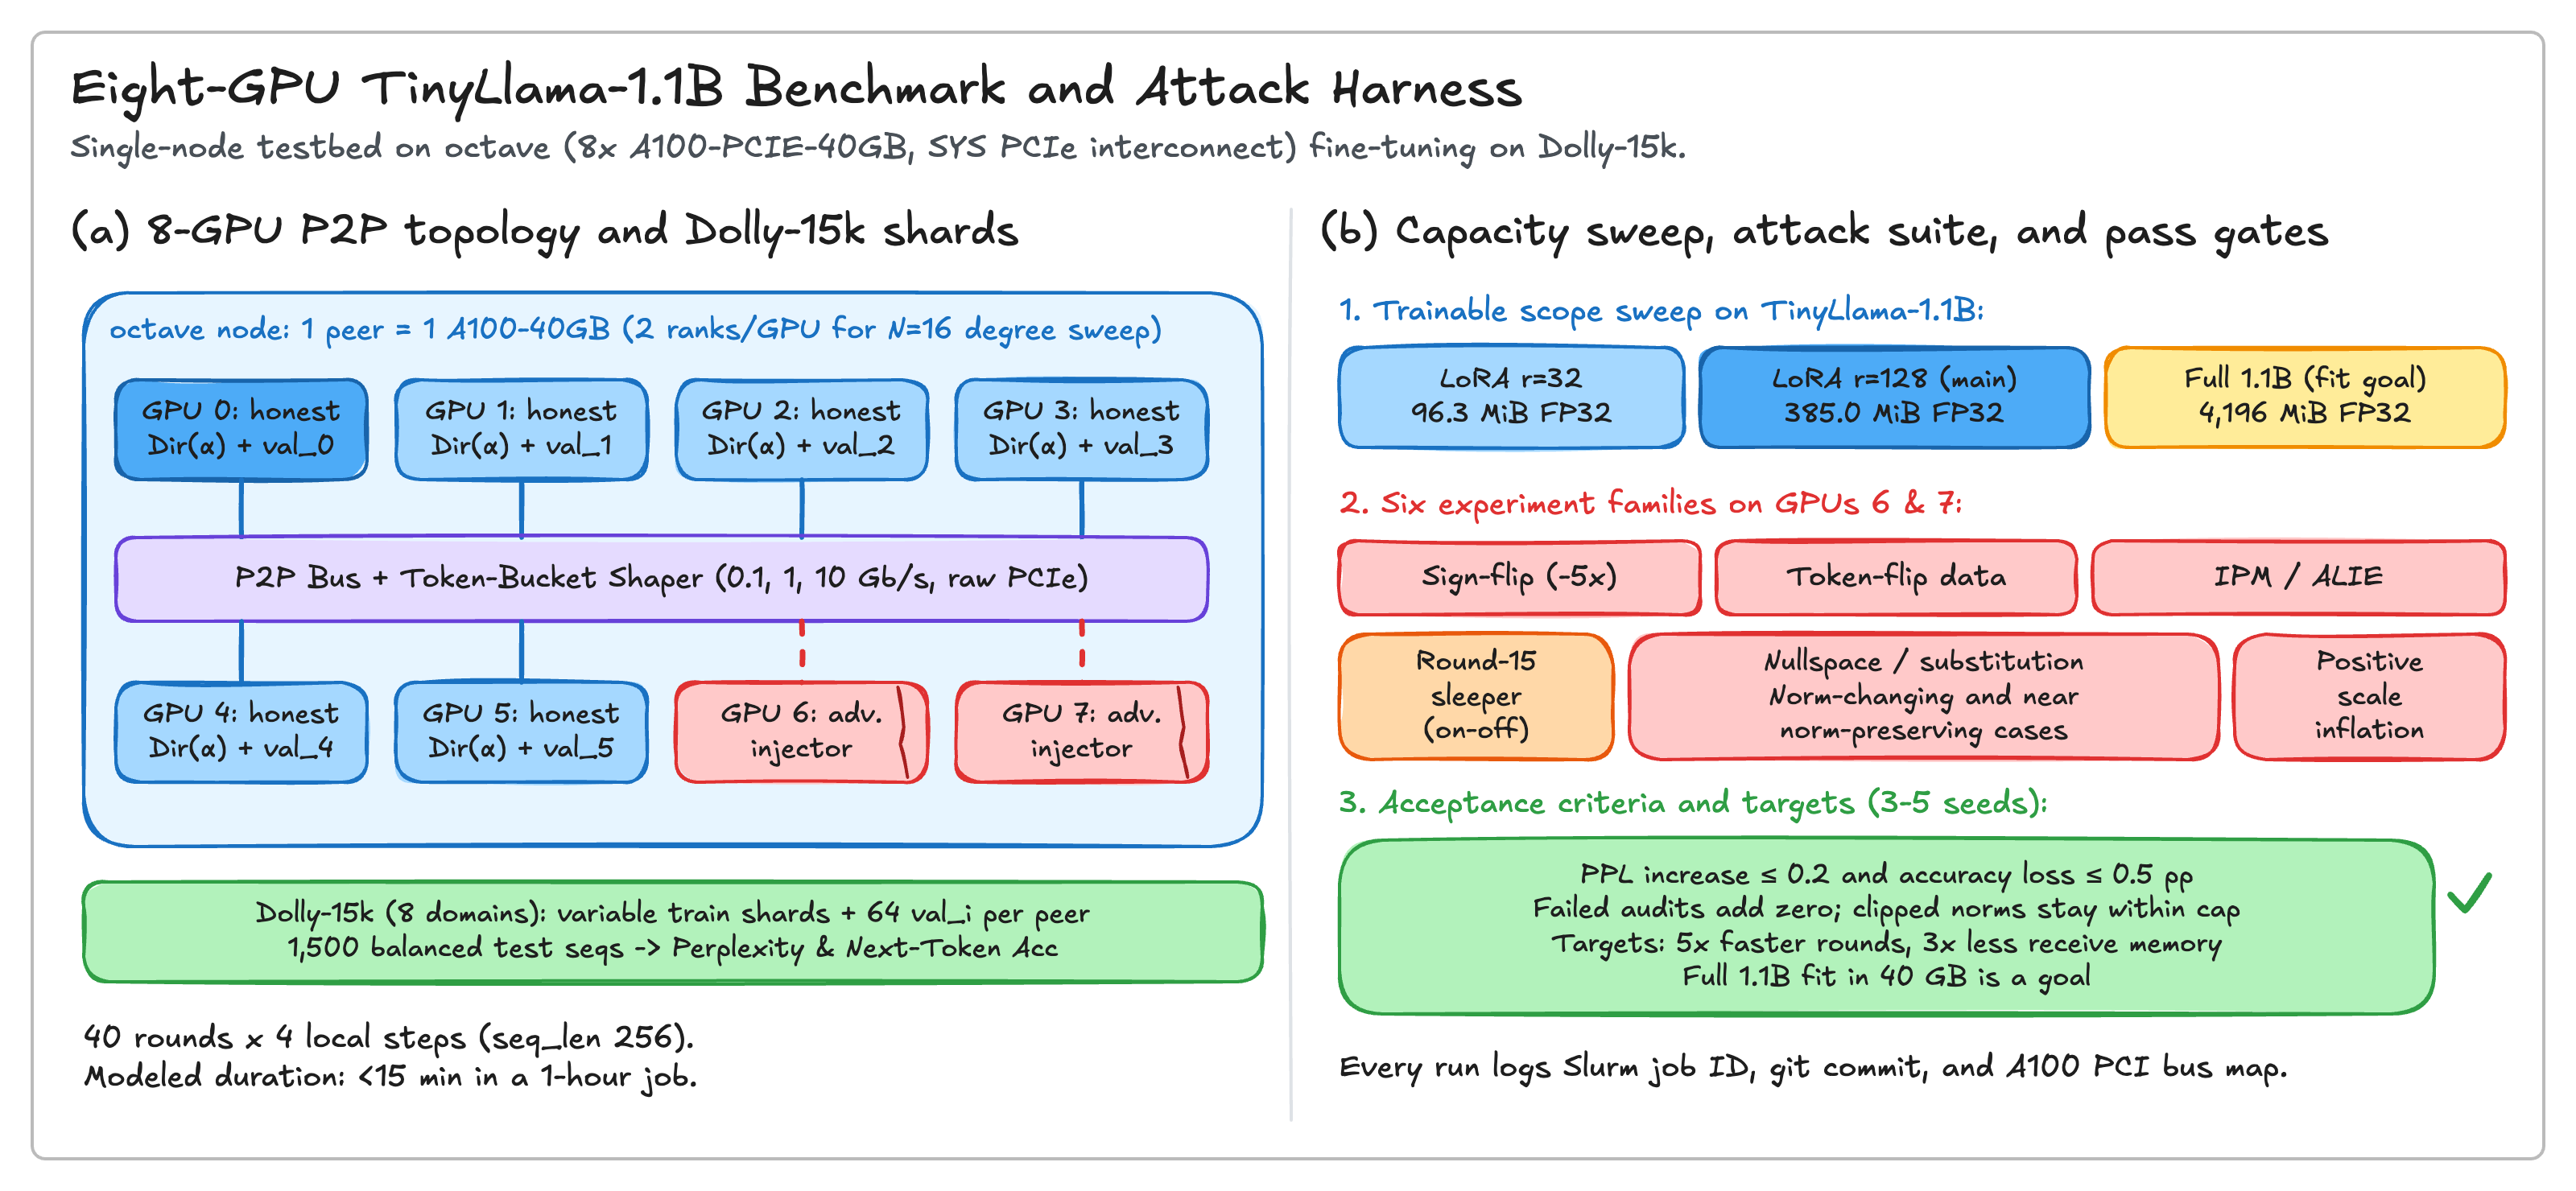
\includegraphics[width=\linewidth]{figures/fig7_eval.png}
  \caption{Eight-GPU evaluation harness. Honest peers train on Dirichlet-partitioned Dolly-15k shards and reserve local validation sequences. Two Byzantine peers exercise six stress families across three trainable scopes.}
  \label{fig:eval}
\end{figure}

Dolly-15k provides roughly $15{,}000$ instruction-response examples in eight categories. We reserve $1{,}500$ category-balanced test examples and allocate the rest by a per-category Dirichlet split. We use concentration $0.1$ by default and also test $0.05$, $0.5$, and IID. Shard sizes vary. We resample splits if a peer has fewer than 80 sequences, enough for 64 validation sequences and one training batch. We report the realized counts. Each sequence is truncated to 256 tokens. The benchmark uses 40 rounds of four AdamW steps at batch size 16 and computes the validation gradient over two batches of 32.

Table~\ref{tab:baselines} lists comparison configurations. The LLM variants use the same transport, starting weights, and data order. We also toggle the sketch gate, streaming, clipping, and quarantine separately to isolate each contribution. A dense streaming baseline separates the effect of buffering from the effect of reducing received bytes.

\begin{table}[tbp]
  \caption{LLM comparison configurations. TrustGraph variants use the descent-corrected sign convention.}
  \label{tab:baselines}
  \centering\small
  \begin{tabularx}{\linewidth}{@{}P{0.44\linewidth}Y@{}}
    \toprule
    Configuration & Experimental role \\
    \midrule
    Unprotected DFL & Reference without Byzantine filtering. \\
    BALANCE & Distance-based decentralized defense without a validation set. \\
    Batched TrustGraph-DFL (FP32) & Primary uncompressed baseline for accuracy and receive costs. \\
    Sparse Top-1\% + TrustGraph & Measures alignment loss from sparsification on non-IID data. \\
    Blockwise INT4 + TrustGraph & Isolates compression without sketch screening, streaming, or quarantine. \\
    PeerSieve without Pass~1 audit & Measures the value of the audit against a gate-only variant. This variant uses sketch weights and still clips payloads using their decoded norm. \\
    PeerSieve (complete system) & Evaluates sketch screening, audited streaming, clipping, and quarantine. \\
    \bottomrule
  \end{tabularx}
\end{table}

\subsection{Attack and Stress Suite}

The main configuration uses two Byzantine peers. We sweep from zero to three and report the observed adversarial degree per receiver. Let $x_j$ be a clean reference update and $\delta$ a perturbation. Equation~\eqref{eq:attacks} describes the sign-flip and nullspace test families in the update space. For encoded payloads we measure any residual sketch difference introduced by quantization rather than assuming the perturbation stays exactly in the nullspace.
\begin{equation}
\begin{aligned}
  x_j^{\mathrm{flip}} &= -\gamma x_j, \\
  x_j^{\mathrm{null}} &= x_j+\delta, \qquad \mathcal S_t(\delta)=0 .
\end{aligned}
\label{eq:attacks}
\end{equation}

\begin{enumerate}
  \item \textbf{Sign flip.} Negate an update and amplify it fivefold.
  \item \textbf{Token-flip data poisoning.} Permute target response tokens in the Byzantine peers' training data.
  \item \textbf{Inner-product manipulation.} Test updates near the filter's zero-alignment decision boundary.
  \item \textbf{Sleeper.} Use honest updates for rounds 1--14, then switch to sign flipping in round 15.
  \item \textbf{Nullspace and substitution.} Compare norm-increasing and near-norm-preserving cases against a payload whose canonical sketch conflicts with the announced one. Record acceptance rather than assume rejection.
  \item \textbf{Positive scale inflation.} Compare the magnitude of accepted updates with and without clipping under large positive rescaling. Record the realized scale after encoding.
\end{enumerate}

\subsection{Measurements and Acceptance Criteria}

For each configuration and stress case, we record held-out perplexity and next-token accuracy, honest rejection, Byzantine acceptance and aggregate weight, bytes received, phase times, and peak CUDA memory. We log the cause of each audit rejection and track the largest honest connected component as well as observed active degree. We separate local training, validation, encode and sketch, network wait, and audit time. We run convergence at $1$~Gb/s and ten-round timing runs at $100$~Mb/s, $10$~Gb/s, and unthrottled PCIe. Each configuration and attack uses three to five paired seeds, with an untimed warm-up and median and range reported across seeds. We record the Slurm job ID, git commit, and GPU PCI bus map for each run.

In the receive-memory model, $D$ is the size in MiB of a dense FP32 update and $Q$ is the compressed size in MiB. The batched baseline holds $(K+2)D$~MiB: one dense update per neighbor, the validation vector, and the accumulator. PeerSieve holds $(2D+Q+4)$~MiB, plus small sketch buffers and state not included in the table. Table~\ref{tab:vram} models each peer. We use up to two ranks per GPU for the degree sweep and measure end-to-end full-parameter fit separately at degree six with one rank per GPU.

\begin{table}[tbp]
  \caption{Predicted receive-side tensor memory in MiB. Training allocations, sketch bookkeeping, and the sender's FP32 error-feedback residual are excluded.}
  \label{tab:vram}
  \centering\small
  \begin{tabularx}{\linewidth}{@{}Yrrrr@{}}
    \toprule
    Trainable scope & FP32 $D$ & Baseline $K=6$ & Baseline $K=12$ & PeerSieve \\
    \midrule
    Rank-32 LoRA & 96.3 & 770.0 & 1,347.5 & 208.9 \\
    Rank-128 LoRA & 385.0 & 3,080.0 & 5,390.0 & 823.6 \\
    Full 1.1B & 4,196.4 & 33,570.8 & 58,748.9 & 8,937.6 \\
    \bottomrule
  \end{tabularx}
\end{table}

For full-parameter tuning, PeerSieve's receive-side estimate is 8.73~GiB and its separate FP32 residual costs 4.10~GiB. If the remaining training footprint is 18~GiB, the total is about 30.8~GiB before other overheads. We will measure the actual peak, including training state, allocations, and allocator effects, before claiming a fit.

The complete system must meet the following goals in the proposed evaluation:
\begin{enumerate}
  \item \textbf{Accuracy.} Under each tested stress case, final perplexity is no more than $0.2$ above the FP32 baseline and next-token accuracy is no more than $0.5$ percentage points below it.
  \item \textbf{Robustness.} Failed audits never modify the aggregate and accepted payloads respect the norm cap. The honest rejection rate exceeds the baseline's by at most five percentage points. Report any accepted Byzantine payloads and their effect on test metrics.
  \item \textbf{Efficiency.} At degree six with rank-128 LoRA and $1$~Gb/s, median round time is at most one fifth of the batched FP32 baseline's, and measured receive-side tensor memory is at most one third of the baseline's.
  \item \textbf{Scale.} Full-parameter tuning at degree six completes on one 40~GB A100 per peer without running out of memory.
\end{enumerate}

The modeled 9.6$\times$ round-time and 3.7$\times$ receive-buffer improvements are specific to the scenario in Table~\ref{tab:round}. Slower local training, sketch false positives, or the cost of deterministic reductions and two-pass decoding may reduce the gains.

\section{Risks and Limitations}

\textbf{Adaptive updates.} A sketch is not a proof of provenance. Clipping prevents unbounded amplification but does not prevent a peer from selecting a harmful direction or obtaining a large fraction of the trust weight. Accepting consistent Byzantine updates remains possible.

\textbf{Calibration under heterogeneity.} Validation directions may differ across honest peers. Low or negative scores can discard helpful updates even with the correct sign. We will measure these errors by scope, layer, and seed before changing the tolerances. Larger sketches may reduce error at a higher communication cost.

\textbf{Connectivity and synchronization.} Reversible probation and referrals help only when acceptable peers are reachable. PeerSieve does not solve eclipse attacks or remove synchronous straggler delays.

\textbf{Training and validation assumptions.} We assume each honest node's validation split is clean. The memory and timing projections are analytical budgets. The proposed GPU experiments must establish whether the savings hold under the actual training footprint and transport overhead.

\clearpage
\bibliographystyle{unsrtnat}
\bibliography{references}
\end{document}
